\documentclass[oneside,10pt]{book}

\usepackage{cdtBook}
\usepackage{usecases}
\usepackage{requerimientos/requisitos}
\usepackage{amsmath}
\usepackage{amssymb}
\usepackage{booktabs}
\usepackage{hyperref}
\usepackage{enumerate}
\usepackage{mensajes/msg_style}
\usepackage{pdfpages} %Para cargar pdfs
\usepackage{estilos/estilos}
%\overfullrule=2cm

%\title{Análisis}
%\subtitle{}
%\author{Autores: \\Fernández Quiñones Isaac\\Huerta Martínez Jesús Manuel\\Pérez García José David}
%\organization{Escuela Superior de Cómputo, IPN}

%%%%%%%%%%%%%%%%%%%%%%%%%%%%%%%%%%%%%%%%%%%%%%%%%%%%%%%%%%%%%%%%
\begin{document}

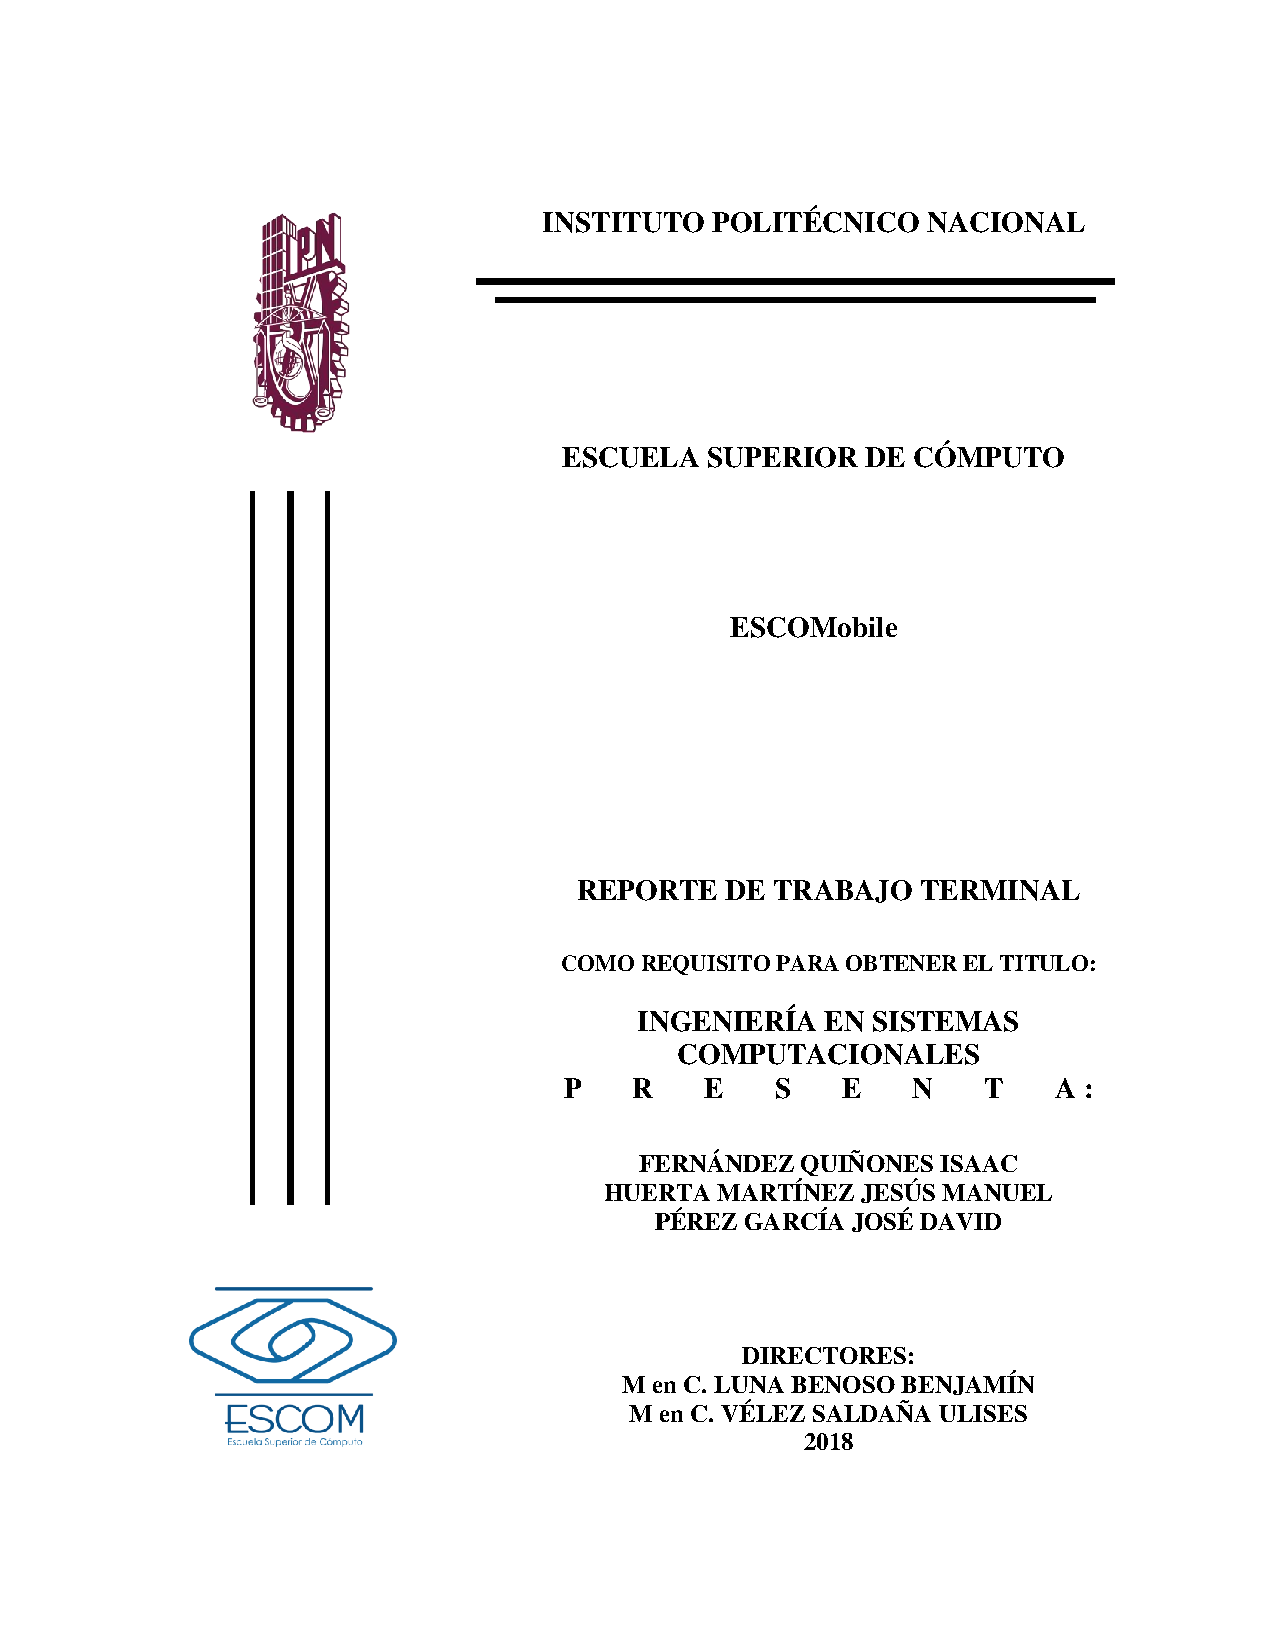
\includepdf[pages=1]{portada/posible_portada}

%\maketitle
%\thispagestyle{empty}
\frontmatter
\tableofcontents
\listoffigures
\listoftables
\mainmatter

%=========================================================
%                                                         INTRODUCCIÓN.
%=========================================================

\chapter{Introducción}

% Introducción.
\cfinput{intro/Introduccion}
% Justificación.
\cfinput{intro/Justificacion}
% Objetivos.
\cfinput{intro/Objetivos}

%=========================================================
%                                                 TÉRMINOS DEL NEGOCIO.
%=========================================================

\chapter{Términos del negocio}
\cfinput{marco_teorico/glosario}

%=========================================================
%                                                 	        ANTECEDENTES.
%=========================================================

\chapter{Antecedentes}

% Marco teórico.
\cfinput{antecedentes/marco_teorico}
% Propuesta.
\cfinput{antecedentes/propuesta}
% Estado del arte.
\cfinput{antecedentes/estadoarte}
% Trabajo realizado en tt1. 
\cfinput{antecedentes/trabajo_ttuno}
% Observaciones tt1.

%=========================================================
%                                                            REQUISITOS.
%=========================================================

\chapter{Requisitos de software}

% Requerimientos.
\cfinput{requerimientos/requisitos}
% Tecnologías a usar.
\cfinput{requerimientos/tecnologias}

%=========================================================
%                                                   ANALISIS DE RIESGOS.
%=========================================================

\chapter{Analisis de Riesgos}
\cfinput{riesgos/analisisderiesgos}

%=========================================================
%                                                MODELO DE INTERACCION
%=========================================================

\chapter{Modelo de la Interacción}

\noindent
En este apartado se muestran las diferentes pantallas que componen a la aplicación ESCOMobile,
la forma en que éstas se estructuran y la descripción de las diferentes secciones que las componen.
La información que se puede consultar en la descripción incluye: objetivo, descripción del diseño, 
una imagen que ilustra el diseño descrito, las entradas requeridas (de ser el caso) y las salidas
generadas y mostradas dentro de la propia pantalla, así como los comandos y mensaje con las que
éstas pueden llegar a contar.

\noindent
\newline
A continuación, se muestra la descripción de cada una de las pantallas que forman ESCOMobile,
en el mismo orden del cual se descibieron los casos de uso.

% Pantallas.
\cfinput{Pantallas/Acceso/UI_Acceso}
\cfinput{Pantallas/Mapa/UI_Mapa}
\cfinput{Pantallas/Alumno/UI_Alumno}
\cfinput{Pantallas/AlumnoBolsa/UI_AlumnoBolsa}
\cfinput{Pantallas/AlumnoProfesor/UI_AlumnoProfesor}
\cfinput{Pantallas/Profesor/UI_Profesor}
\cfinput{Pantallas/Citas/UI_Citas}
\cfinput{Pantallas/BolsaWeb/UI_WebBolsa}

%=========================================================
%                                                                MENSAJES.
%=========================================================

\chapter{Modelo de mensajes}
\cfinput{mensajes/mensajes}

%=========================================================
%                                                              BIBLIOGRAFIA.
%=========================================================

\cfinput{bibliografia/bibliografia}

% FIN DEL DOCUMENTO.
\end{document}
